\documentclass[a4paper,11pt]{article}
%\pdfoutput=1 % if your are submitting a pdflatex

\usepackage{jheppub} % see the JHEP-author-manual
\usepackage[utf8]{inputenc} % 
\usepackage{xfrac}
\usepackage{ulem}   % TO REMOVE
\usepackage{xcolor}
\usepackage[title]{appendix}
%\usepackage[page,toc,titletoc,title]{appendix}
\usepackage{tocloft}
\pagenumbering{arabic}



\usepackage{hyperref}
\hypersetup{
    colorlinks=true,  
    linktoc=all,     %set to all if you want both sections and subsections linked
    linkcolor=blue,  %choose some color if you want links to stand out
    filebordercolor=red,
    linkbordercolor=blue, 
    urlbordercolor=green,
    citebordercolor=green,
    pdftitle={Topology and phase transition},
    pdfauthor={A.Haddad},
}

\usepackage[
backend=biber,
style=numeric,%alphabetic
sorting=ynt
]{biblatex}
\addbibresource{biblio.bib}
%%%%%%%%%%%%%%%%%%%%%%%%%%%%%%%%%%%%%%%%%%%%%%%%%%%%%%%%%%%%%%%%%%%%%%%%%%%%%%%%%%%%%%%%%%%%%%%%%%%%%%%%%%%%%%%%%%%%%%%%%%%%%%%

\titre{\boldmath Conceptual introduction to BKT transition in the XY model, glimpse into topological point of view}%Conceptual introduction to Topological theory of Phase Transitions
\UE{Work presented to complete the scientific watch course}
\sujet{Master FunPhys M1 - semester 2 -} 

\enseignant{
\href{mailto:pettini@cpt.univ-mrs.fr}{Pr. Marco \textsc{Pettini}}
}

\eleves{%Nom de l'élève
\href{mailto:abdelhamid.haddad@etu.univ-amu.fr}{Abdelhamid \textsc{Haddad}}
}

\normalsize
\abstract{Phase transition have always been a huge topic of interest in theoretical and experimental physics, we report in this papaer a short conceptual introduction to the topological treatement of phase transition, trying to retrace it from the well know Laudau theory, the mermin-wagner theorem, XY model and it's explanation as given by the so-called Berezinsky-Kosterlitz-Thouless phase transition and we ended by introducing the seminal idea of topological phase transition.}
\keywords{Phase transition, XY model, Berezinsky-Kosterlitz-Thouless phase transition, Topological hypothesis in phase transition}


%%%%%%%%%%%%%%%%%%%%%%%%%%%%%%%%%%%%%%%%%%%%%%%%%%%%%%%%%%%%%%%%%%%%%%%%%%%%%%%%%%%%%%%%%%%%%%%%%%%%%%%%%%%%%%%%%%%%%%%%%%%%%

\usepackage{fancyhdr}
\pagestyle{fancy}
\fancyhf{}
\begin{document}

\pagedegarde

\setcounter{page}{2}

\ifnotoc\else
\iftoccontinuous\else\newpage\fi
\beforetochook\hrule
\tableofcontents
\afterTocSpace
\hrule
\afterTocRuleSpace
\fi


\section{Introduction}

In 1937, \textit{Lev Davidovitch Landau} proposed a phenomenological theory to describe (second-order) phase transitions (PT) \cite{landau1937theory}, it was succesfully and universaly applied to describe Ising model, superconductivity throughout the so-called Landau-Ginzburg theory \cite{ginzburg2009theory}, and was at the origin of Renormalization Group \cite{kadanoff1966scaling,wilson1975renormalization} : largely used in quantum field theories.


Intuitively, PT can be understood as a qualitative physical changes on a many-body system that happen in any scale, ranging from confinement/deconfinement at the nuclear level \cite{wilson1974confinement} up to the clustering of galaxies \cite{cerruti2001clustering}. In short, the leading theory of Landau goes like that: 

\begin{center}\textit{"
When a continuous phase transition occurs in a physical system by cooling below a critical temperature $T_c$, the internal symmetry of the system is reduced (broken). Knowledge of the symmetries above and below $T_c$, encapsulated in a bosonic order parameter, uniquely specifies the properties of the phase transition, in particular the critical exponents. As a result, transitions in very diverse physical systems (e.g., the transition from normal to superfluid helium and from a para- to a ferromagnet) are captured by a single universal theory if their symmetries match."}\cite{Alsolami2012Auth}
\end{center}


In this simplicity, the story sounds almost too good to be true ! And a whole machinery of critical exponents around critical point, universality classes and much more ideas that aren't in the scope of this work. From this, you may think that we are pretty done with PT and there no much more to see ? unfortunately, and as is usually the case in theoretical physics, things aren't too simple. We will explore in next section one of the limitation of this theory known as the XY model.



As a last remark, at the beginning of this work, we was facing a trouble and a little bit of confusion with Topological quantum matter, so here is the point : We have to make a clear difference between Topological quantum matter that treat about the change of the behavior of the matter itself, in real space, whereas, by topological phase transition we meant the change of the topology in phase space, note that the mathematical tools used in both of them are pretty similar, namely \textit{Topology}, \textit{Gauss-Bonnet theorem}, ect\footnote{Interested reader may consult \href{https://wwwphy.princeton.edu//~haldane/research.html}{theses conferences by Pr.Duncan Haldane} for more details.}.


\section{Mermin-Wagner theorem} 

In the seminal papers \cite{mermin1966absence,hohenberg1967existence}, it was shown that 

\begin{center}\textit{"
In one and two dimensions, continuous symmetries cannot be spontaneously broken at finite temperature in systems with sufficiently short-range interactions."} \cite{wagner} 
\end{center}

This is known as the \textit{Mermin-Wagner Theorem} and a short demonstration can be found in \cite{wagner}. An important remark is that the theorem is restricted only to the non-existence of spontaneous magnetization. It does not necessarily exclude other types of phase transitions. For example the magnetic susceptibility may diverge as it will be relevant for what follow next.

So, based on Landau theory and taking into account the Mermin-Wagner theorem, we may conclude that for a 2d system with a continuous symmetry, and as there is no possible breaking symmetry, thet can't be a phase transition ! In what follow, we will aboard briefly the well-known XY model that exhibit a phase transition without any symmetry breaking. 

\section{BKT transition and the XY model}
\subsection{The XY model}

The XY model is a two-vector model on a two-dimensional lattice, where in every site we associate a two-dimensional
unit-vector $S_i~=~(\cos(\theta_i),\sin(\theta_i))$ and the Hamiltonian read:

\begin{equation}
H_{XY}= -J~\sum_{i}^N \cos(\theta_i - \theta_{j}),
\label{Hxy}
\end{equation}

This system is rotationally invariant (i.e., symmetric under $\theta_i~\rightarrow~\theta_i~+~c$) and the sum is over closer neighbors.

In condensed matter physics we classify matter in 3 basic states, in terms of the decay of their correlation functions \cite{correlation} :

\begin{equation}
G(x,x')=
\begin{cases}
\text{Long range ordered state} &\text{if} \rightarrow~c~\neq~0\\
\text{Disordered state : Exponential decay} &\text{ if $\xrightarrow{\propto exp(|x-x'|)} 0$}\\
\text{Quasi long range ordered state : Algebraic decay} &\text{ if $\xrightarrow{\propto |x-x'|^{-\eta}} 0$}
\end{cases}
\label{corrr}
\end{equation}

Where jumping from one state to another defines a phase transition for the system.

It was shown\footnote{It can be found in the litterature, for example in \cite{correlation} and \cite{corr2}} that the low temperature phase of the 2D XY model is quasi-long-range-ordered, whereas at the high temperature regime, it exhibit a . Therefor, it is interesting to ask how the phase transition may be possible between the quasi-long-range-ordered to a disordered state without breaking any symmetry !

We usually associate a phase transition with a process of a symmetry breaking, but here neither of the phases breaks any symmetry, so one naively expects not to find a transition. As it turns out, there is a transition, and it is called the Berezinskii-Kosterlitz-Thouless transition. Historically, it was the first example of a topological phase transition.

\subsection{The Berezinsky, Kosterlitz, Thouless PT}

The explanation of Berezinsky, Kosterlitz and Thouless was congratulated in 2016 by the Nobel prize and goes as follow \cite{kosterlitz1973j}: 

\begin{itemize}

\item At low temperatures the system contain a dilute ‘gas’ of vortex-antivortex pairs, each vortex will stick to an antivortex, since it takes a lot of energy to separate them.

\item As you heat up the system, you get more and more vortex-antivortex pairs, since there’s more energy available to create them. 

\item At high temperature, the density of vortex-antivortex pairs is so high, and they’re bumping into each other so much, that we can’t tell which vortex is the partner of which antivortex. All we’ve got is a thick soup of vortices and antivortices.

\end{itemize}

What’s interesting is that this happens suddenly at some particular temperature. A sudden change in behavior like this is called a phase transition. So, the Kosterlitz–Thouless transition is the sudden unbinding of the vortex-antivortex pairs as you heat up your system.


\section{Topological hypothesis}

As the study of phase transition lack a general and universal theoretical framwork that can be applied equivalently between systems without any distinction, so in order to understand in a better way phase transitions, it was argued in \cite{caiani1997geometry} that 

\begin{center}\textit{
“A thermodynamic transition might be related to a change in the topology of the configuration space, and the observed singularities in the statistical-mechanical equilibrium measure and in the thermodynamic observables at the phase transition might be interpreted as a “shadow” of this major topological change that happens at a more basic level.”}
\end{center}

In other words, it is conjectured that the phase transition might correspond to a change in the topology of the manifolds whose geodesics are the motions of the system. Here we have choose to show how it was applied to the previously disscussed case of BKT in the XY model, but keep in mind that the idea is more general and expected to be applied for any systems performing a phase transition. 


In order to do, thet have studied the Hamiltonian dynamics associated with classical Heisenberg XY models as it was investigated in \cite{cerruti2000hamiltonian,Caiani_1997} by the addition to the Heisenberg potentials of a standard quadratic kinetic energy term.%In fig.\ref{1},we have represented the Largest Lyapounov exponent with respect to the energy density : 

%\begin{figure}[htbp]
%\centerline{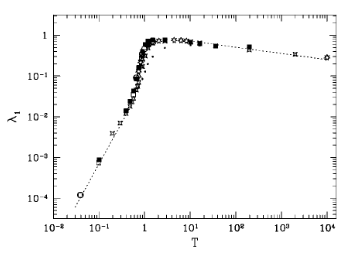
\includegraphics[scale=.5]{lyapounov.png}}
%\caption{Lyapunov exponent vs energy density for the XY model as taken from \cite{Caiani_1997}.}
%\label{1}
%\end{figure}

Again, this point of view is not completely well defined and then have to be taken carefully, a topological changes in phase space cannot always be linked to a phase transition in realm, interested reader may follow \cite{marco:hal-01260170} for more intriguing discussions.

\section{Summary and perspectives}

Even if we wasn't too much into the details on what we presented above, remind that our goal was to retrace a bit the conceptual ideas that attemp to understand phase transitions up to the topological point of view. We aim that it was enough to let the reader become more interested into this topic, and we hope we have succeeded. We summararize here naively waht we leaned all along this work and give a hint to potential future work that can be done:

\begin{enumerate}
\item In two dimension, continuous spin models cannot have magnetically ordered state (Mermin-Wagner theorem).

\item However, the XY model, which is a two-dimentional continuous spin model, has a strange type of PT that does not break any symmetry as argues by Landau theory, but exhibit a change in the topology itself as succesfully explained by the creation of Vortex/Antivortex by increasing the temperature, up to a a certain "critical" temperature that will cause thoses Vortex/Antivortex to unbine from each other suddenly, this explanation is largely know as the \textit{Berezinsky, Kosterlitz, Thouless phase transition} (BKT).

\item Even if the topological point of view presented above may provide a new theoretical tool to tackle PT (topological hypothesis), is still lack of a complete description of it and in some cases, we may observe a topological change in phase space which doesn't correspond to any phase tansition, even if any phase transition in real space may correspond to a topological "transition" in phase space, so it will be interesting to search on what kinds of topological transitions may be related to a real PT ? what is the missing element of this picture ? 
 
\item A related and intermeadiate questions is to ask, starting from a known first or second order PT in real space, what will be the difference in their topological transition ? is second order phase transition really exist or it is just an artefact ?

\end{enumerate}

\section*{Acknowledgements}

The author warmly acknowledge Pr. Marco Pettini (Aix-Marseille Univ, Université de Toulon, CNRS, Centre de Physique Théorique Marseille) for guiding advises, inspiring mentoring and a huge patience throughout along this work.

%\begin{appendices}
%\setcounter{equation}{0}
%\section{Review of Hamiltonian dynamics}
%\end{appendices}



\addcontentsline{toc}{section}{References}
\printbibliography %Prints bibliography


\end{document}